\documentclass{llncs}

\usepackage{graphicx}
\usepackage{caption}
\usepackage{subcaption}
\captionsetup{compatibility=false}

\usepackage{xcolor}
\usepackage{enumitem,amsmath,amssymb}
\usepackage{breakurl}    % used for \url and \burl
\usepackage[linesnumbered,boxed,noline,noend]{algorithm2e}
\def\defaultHypSeparation{\hskip.1in}

\usepackage{tikz}
%\usepackage{subfig}
\usepackage{array,booktabs,multirow}
\usepackage{placeins}

\usepackage{logictools}
\usepackage{prooftheory}
\usepackage{comment}
\usepackage{mathenvironments}
\usepackage{drawproof}

\DeclareMathOperator{\pebble}{P}
\DeclareMathOperator{\unpebble}{U}
\DeclareMathOperator{\pebbledAt}{pebbledAt}

\newcommand{\indexIn}[3]{\ensuremath{#1 \scriptstyle \in \{#2\ldots #3\} \displaystyle}}

\usetikzlibrary{patterns}

\renewcommand{\topfraction}{0.85}
\renewcommand{\textfraction}{0.1}
\renewcommand{\floatpagefraction}{0.75}

\newcommand{\defeq}{\mathrel{\mathop:}=}
\newcommand{\eqdef}{\mathrel{\mathop=}:}

\newcommand{\nodedistance}{0.55cm}
\newcommand{\nodedistanceThree}{0.6cm}
\newcommand{\nodedistanceTwo}{1.2cm}

\newcommand{\Vertices}[1]{V_{#1}}
\newcommand{\Edges}[1]{E_{#1}}
\newcommand{\Conclusion}[1]{\clause_{#1}}
\newcommand{\Premises}[2]{P_{#1}^{#2}}
\newcommand{\Children}[2]{C_{#1}^{#2}}
\newcommand{\Axioms}[1]{A_{#1}}

\title{Greedy Pebbling: \\ 
Towards Proof Space Compression}

\author{
  Andreas Fellner 
  \thanks{Supported by the Google Summer of Code 2013 program.}
  \and 
  Bruno Woltzenlogel Paleo 
  \thanks{Supported by the Austrian Science Fund, project P24300.}
}

\authorrunning{A.\~Fellner \and B.\~Woltzenlogel Paleo}

\institute{
  \email{fellner.a@gmail.com} \ \ \ \email{bruno@logic.at} \\
  Theory and Logic Group \\
  Institute for Computer Languages \\
  Vienna University of Technology
}

\begin{document}

\maketitle

\begin{abstract}
This paper describes algorithms and heuristics for playing a \emph{Pebbling Game}. Playing the game with a small number of pebbles is analogous to checking a proof with a small amount of available memory. Here this analogy is exploited: new pebbling algorithms are conceived and evaluated on the task of compressing the space of thousands of propositional resolution proofs generated by SAT- and SMT-solvers.
\end{abstract}

\setcounter{footnote}{0}


\section{Introduction}

Proofs generated by SAT-solvers can be huge. 
Checking their correctness can not only take a long time but also consume a lot of memory. 
In an ongoing project for controller synthesis based on the extraction of interpolants from SMT-proofs \cite{Hofferek}, 
for example, post-processing a proof takes hours and may reach the limit of memory available today in a single node of a computer cluster (256GB). This issue is even more relevant in application scenarios in which the proof consumer, who is interested in independently checking the correctness of the proof, might have less available memory than the proof producer.
This is in part because, while the proof checker reads a usual proof file and checks the proof it contains, 
every proof node (containing a clause) that is loaded into memory has to be kept there until the end of the whole proof checking process, 
since the proof checker does not know whether a proof node will still need to be used and re-reading the proof file to reload and recheck proof nodes would be too time-consuming. 

To address this issue, recently proposed proof formats such as DRUP \cite{drup} and BDRUP \cite{bdrup} allow enriching a proof file with instructions that inform a proof checker when a proof node can be released from memory. Other proof formats, such as the TraceCheck format \cite{tracecheck} could also be enriched analogously. Such node deletion instructions can be added by a proof-generating SAT-solver during proof search in the periodic clean-up of its database of derived learned clauses; for every clause the SAT-solver deletes during this phase, this deletion can be recorded in the proof file. 

This paper explores the possibility of post-processing a proof in order to increase the amount of deletion instructions in the proof file. The more deletion instructions, the less memory the proof checker will need. Therefore, this \emph{deletion-during-proof-postprocessing} approach ought to be seen not as a replacement but rather as an independent complement to the \emph{deletion-during-proof-search} already performed by state-of-the-art proof-generating SAT-solvers.

The new methods proposed here exploit an analogy between proof checking and 
playing \emph{Pebbling Games} \cite{kasai1979classes,gilbert1980pebbling}. 
The particular version of pebbling game relevant for proof checking is defined precisely in Section \ref{sec:pebbling-game} and the analogy to proof checking is explained in detail in Section \ref{sec:pebblingchecking}. The proposed pebbling algorithms are greedy (Section \ref{sec:algorithms}) and based on heuristics (Section \ref{sec:heuristics}). As discussed in Sections \ref{sec:pebblingchecking} and \ref{sec:PebblingAsSat}, approaches based on exhaustive enumeration or on encoding as a \emph{Sat} problem would not fare well in practice.

The proof space compression algorithms described here are not restricted to proofs generated by SAT-solvers. They are general DAG pebbling algorithms, that could be applied to proofs represented in any calculus where proofs are directed acyclic graphs (including the special case of tree-like proofs). It is, nevertheless, in \emph{Sat} and \emph{SMT} that proofs tend to be largest and in most need of space compression. The underlying propositional resolution calculus (described in Section \ref{sec:Resolution}) satisfies the DAG requirement. The experiments (Section \ref{sec:exp}) evaluate the proposed algorithms on thousands of SAT- and SMT-proofs.


\section{Propositional Resolution Calculus}
\label{sec:Resolution}

A \emph{literal} is a propositional variable or the negation of a propositional variable. The
\emph{complement} of a literal $\ell$ is denoted $\dual{\ell}$ (i.e. for any propositional variable $p$,
$\dual{p} = \neg p$ and $\dual{\neg p} = p$). The set of all literals is denoted $\mathcal{L}$. A
\emph{clause} is a set of literals. $\bot$ denotes the \emph{empty clause}.


\newcommand{\axiom}[1]{\widehat{#1}}
\newcommand{\n}{v}
\newcommand{\raiz}[1]{\rho(#1)}

\begin{definition}[Proof] 
\label{def:proof}
A \emph{proof} $\varphi$ is a tuple $\langle V,E,\n,\clause \rangle$, 
such that $\langle V,E \rangle$ is a directed acyclic graph whose edges are labeled with literals $\ell \in \mathcal{L}$, $\n \in V$, $\clause$ is a clause 
and one of the following holds:

\begin{enumerate}
	\item $V = \{\n\}, E = \emptyset$
	\item \label{enum:resCase} There are proofs $\varphi_L = \langle V_L, E_L, \n_L,\clause_L \rangle$ and $\varphi_R = \langle V_R, E_R, \n_R, \clause_R \rangle$ such that 
	    \begin{align*}
			\n & \text{ is a new node} \\
      V &= V_L \cup V_R \cup \{\n \} \\
      E &= E_L \cup E_R \cup
                    \left\{\n_L \xrightarrow{\dual{\ell}} \n , \n_R \xrightarrow{\ell} \n \right\} \\
     \Gamma &= \left( \clause_L \setminus \left\{ \dual{\ell} \right\} \right) \cup \left( \clause_R
                    \setminus \left\{ \ell \right\} \right)
    \end{align*}
		$\n$ is called the \emph{root} of $\varphi$ and $\clause$ its \emph{conclusion}.\\
		In case \ref{enum:resCase} $\varphi_L$ and $\varphi_R$ are called \emph{premises} of $\varphi$ and $\varphi$ is called a \emph{child} of both $\varphi_L$ and $\varphi_R$.
		The transitive closure of the premise relation is the \emph{subproof} relation. A subproof which
		has no premises is an \emph{axiom} of the respective proof.
		$\Vertices{\varphi}$ and $\Axioms{\varphi}$ denote, respectively, the set of nodes and axioms of $\varphi$. $\Premises{\n}{\varphi}$ denotes the premises and $\Children{\n}{\varphi}$ the children of the subproof with root $\n$ in a proof $\varphi$. When a proof is represented graphically, the root is drawn at the bottom and the axioms at the top. The \emph{length} of a proof $\varphi$ is the number of nodes in $\Vertices{\varphi}$ and is denoted $\plength{\varphi}$.
\qed
\end{enumerate}

\end{definition}

\noindent
Note that in case \ref{enum:resCase} of definition \ref{def:proof} $V_L$ and $V_R$ are not required to be disjunct. Therefore the underlying structure of proofs are DAGs as opposed to simple trees. Modern SAT- and SMT-solvers produce proofs of such kind \cite{BoutonCaminha-B.-de-OliveiraDeharbeFontaine2009veriT:-an-open-trustable-and-efficient-SMT-Solver,marques2009conflict} and the reuse of proof nodes plays a central role in proof compression \cite{fontaine2011compression}.\\
Also note that a DAG corresponding to a proof by definition has exactly one sink, also called its root node.\\
From hereon, if free from ambiguity, proofs and their underlying DAGs will not be distinguished. For example a node of a proof $\langle V,E,\n,\clause \rangle$ will be meant to be some $s \in V$.

\section{Pebbling Game}
\label{sec:pebbling-game}

%Todo: Discuss relation to resolution space complexity further
Pebbling games were introduced in the 1970's to model programming language expressiveness \cite{paterson1970comparative,Walker1973404} and compiler construction \cite{sethi1975complete}. More recently, pebbling games have been used to investigate various questions in parallel complexity \cite{chan2013pebble} and proof complexity \cite{ben2008short,Esteban200184,nordstrom2009narrow}. They are used to obtain bounds for space and time requirements and trade-offs between the two measures \cite{van1979move,ben2009size}. In this paper we investigate space requirements when time is fixed.\\
\textit{To pebble} a node is to put a pebble on it; \textit{to unpebble} is to remove a pebble; a node is \textit{pebbleable} if it is not pebbled but can be pebbled.

\begin{definition}[Static Pebbling Game]
\label{def:pebbling-game}
The \emph{Static Pebbling Game} is played by one player on a DAG $G = (V,E)$ with one distinguished node $s \in V$.
The goal of the game is to pebble $s$, respecting the following rules:
\begin{enumerate}
	\item \label{rule:premises} A node $\n$ is pebbleable \emph{iff} all predecessors of $\n$ in $G$ are pebbled.
	\item \label{rule:unpebbling} Nodes can be unpebbled at any time.
	\item \label{rule:onlyonce} Once a node has been unpebbled, it can not be pebbled again later.
\end{enumerate}
\qed
\end{definition}

Note that as a consequence of rule \ref{rule:premises}, pebbles can be put on nodes without predecessors at any time.\\
Also note that rule \ref{rule:onlyonce} corresponds to fixing the time required to play the game, as with this rule the number of moves will be $O(n)$.

\begin{definition}[Strategy]
\label{def:strategy}
A \emph{pebbling strategy} for the Static Pebbling Game, played on a DAG $G = (V,E)$ and distinguished node $s$, is a sequence of moves $(m_1,\ldots,m_n)$, such that the following formula corresponding to the rules and the goal of the game, using the predicates $\pebble(.)$ and $\unpebble(.)$, is true:
\begin{gather*}
	m_n = \pebble(s) \enskip \wedge \\
	\Big( \forall \indexIn{i}{1}{n}: m_i = \pebble(\n) \Rightarrow \\
																\big( \forall \indexIn{k}{i+1}{n}: m_k \neq \pebble(\n) \wedge \forall o \in \Premises{\n}{G}: \pebbledAt(i,o,m^n_1) \big) \Big) \enskip \wedge\\
	\big( \forall \indexIn{i}{1}{n}: m_i = \unpebble(\n) \Rightarrow \pebbledAt(i,\n,m^n_1) \big)\\[1ex]
	\text{where } \pebbledAt(i,\n,m^n_1) := \exists \indexIn{j}{1}{i-1}: \left( m_j = \pebble(\n) \wedge \forall \indexIn{l}{j}{i-1}: m_l \neq \unpebble(\n) \right)
\end{gather*}
%\begin{align*}
	%m_i = \pebble(\n) &\text{ then for all predecessors }p \text{ of }\n there exists a j: 1 \leq j < i, such that m_j = \pebble(p) and for all l: j < l < i	holds m_l \neq \unpebble(s)\\
	 %& and for all k \in \{i+1,\ldots,n\} holds m_k \neq \pebble(\n)\} \\
	 %m_n = \pebble(s) & \\
%\end{align*}
\end{definition}

In the formula above $\Premises{\n}{G}$ denotes, similarly as defined for proofs, the set of predecessors of $\n$ in $G$.
The following definition allows to measure how many pebbles are required to play the Static Pebbling Game on a given graph.

\begin{definition}[Pebbling number]
The \emph{pebbling number of a pebbling strategy} $(m_1,\ldots,m_n)$ is defined as 
$$
	max_{\indexIn{i}{1}{n}}(|\{\n \in V \mid \pebbledAt(i,\n,m^n_1)\}|)
$$
where $\pebbledAt(i,\n,m^n_1)$ denotes the same formula as in definition \ref{def:strategy}.\\
The \emph{pebbling number of a DAG $G$ and node $s$} is defined as the minimum pebbling number of all pebbling strategies for $G$ and $s$.
\end{definition}

Note that the definitions \ref{def:pebbling-game} and \ref{def:strategy} leave freedom when to do unpebbling moves.
With the aim of finding strategies with low pebbling numbers, there is a canonical way when to do these moves, as will be shown later.

\noindent
The \emph{Static Pebbling Game} from definition \ref{def:pebbling-game} slightly differs from the Black Pebbling Game discussed in \cite{hertel2007black,pippenger1982advances} in two aspects. Firstly, the Black Pebbling Game does not include rule \ref{rule:onlyonce}. Not having this rule allows for pebbling strategies with lower pebbling numbers (\cite{sethi1975complete} has an example on page 1), but at a possible cost of exponentially more moves \cite{van1979move}. Secondly, when pebbling a node in the Black Pebbling Game, one of its predecessors' pebbles can be used instead of a fresh pebble (i.e. a pebble can be moved). The trade-off when allowing to moving pebbles are discussed in \cite{van1979move}. Deciding whether the pebbling number of a graph $G$ and node $s$ is smaller than $k$ is PSPACE-complete in the absence of rule \ref{rule:onlyonce} \cite{gilbert1980pebbling} and NP-complete when rule \ref{rule:onlyonce} is included \cite{sethi1975complete}.

\section{Pebbling and Proof Checking}
\label{sec:pebblingchecking}

The problem of checking the correctness of a proof while minimizing the memory consumption is analogous to the problem of playing the pebbling game on the proof while minimizing the number of pebbles. Checking the correctness of a node and storing it in memory corresponds to pebbling it. Deleting a node from memory corresponds to unpebbling it. In order to check the correctness of a node, its premises must have been checked before and must still be stored in memory (rule \ref{rule:premises} of the pebbling game). A node that has already been checked can be removed from memory at any time (rule \ref{rule:unpebbling}). The correctness of a node should be checked only once (rule \ref{rule:onlyonce}).

Proof files generated by SAT- and SMT-solvers usually already list the nodes of a proof in a topological order. Even if this were not the case, it is simple to generate a topological order by traversing the proof once.

\begin{definition}[Topological Order]
\label{def:topological-order}
A topological order of a proof $\varphi$ is a total order relation $\prec$ on $\Vertices{\varphi}$, such that 
$
\text{for all } \n \in \Vertices{\varphi} \text{, for all } p \in \Premises{\n}{\varphi}:
p \prec v
$.\\
A pebbling strategy $(m_1,\ldots,m_n)$ \emph{respects} a topological order $\prec$ iff
$$
\forall \indexIn{i}{1}{n}: m_i = \pebble(\n) \Rightarrow \left( \forall \indexIn{j}{1}{i-1}: m_j = \pebble(o) \Rightarrow o \prec \n \right)
$$
\qed
\end{definition}

\noindent
A topological order $\prec$ can be represented by a sequence $(v_1,\dots,v_n)$ of proof nodes, by defining $\prec \defeq \{(v_i,v_j) \mid 1 \leq i < j \leq n\}$. This sequence can be interpreted as a particular pebbling strategy, played on the DAG that corresponds to the proof, that pebbles nodes according to the topological. As already briefly noted in section \ref{sec:pebbling-game}, unpebbling moves are given implicitly by what we call the canonical topological pebbling strategy.

%TODO: remove the ugly k
\begin{definition}[Canonical Topological Pebbling Strategy]
The \emph{canonical topological pebbling strategy} for a proof $\varphi$, its root node $s$ and a topological order $\prec$, represented as a sequence $(v_1,\dots,v_n)$ is defined as follows:
\begin{align*}
m_1 &= \pebble(v_1); k := 0 \\
m_i &= \Bigg\{
\begin{array}{ll}
	\unpebble(v_{i-k}) & \text{iff }\forall o \in \Premises{v_{i-k}}{\varphi}: \pebbledAt(i-k,o,m^{i-1}_1); k := k + 1\\
	\pebble(v_{i-k}) & \text{otherwise}
\end{array}
\end{align*}
where $\pebbledAt(i-k,o,m^{i-1}_1)$ denotes the same formula as in definition \ref{def:strategy}.\\
\qed
\end{definition}

\begin{theorem}
\label{theorem:canonical}
The canonical pebbling strategy has the minimum pebbling number among all pebbling strategies respect the topological order $\prec$.
\end{theorem}
\begin{proof} (Sketch)
All the pebbling strategies respecting $\prec$ differ only w.r.t. their unpebbling moves.
Consider the unpebbling of an arbitrary node $v$ in the canonical pebbling strategy. Unpebbling it later could only possibly increase the pebble number. To reduce the pebble number, $v$ would have to be unpebbled earlier than some preceding pebbling move. But, by definition of canonical pebbling strategy, the immediately preceding pebbling move pebbles the last child of $v$ w.r.t. $\prec$. Therefore, unpebbling $v$ earlier would make it impossible for its last child to be pebbled later without violating the rules of the game.
\qed
\end{proof}

\noindent
Theorem \ref{theorem:canonical} shows that, in the version of the pebbling game considered here, the problem of finding a strategy with a low pebble number can be reduced to the problem of finding a topological order whose canonical strategy has a low pebble number. Unpebbling moves can be omitted, because the optimal moment to unpebble a node is immediately after its last child has been pebbled.

Assuming that nodes are approximately of the same size, the maximum memory needed to check a proof is proportional to the maximum number of nodes that have to be kept in memory while checking the proof according to a given topological order. Thus memory consumption can be estimated by the following measure:

\newcommand{\pspace}[2]{s(#1,#2)}
\begin{definition}[Space]
\label{def:space measure}
The \emph{space} $\pspace{\varphi}{\prec}$ 
of a proof $\varphi$ and a topological order $\prec$ is the pebbling number of the canonical topological pebbling strategy of $\varphi$, its root and $\prec$.
\qed
\end{definition}

\noindent
The problem of compressing the space of a proof $\varphi$ and a topological order $\prec$ is the problem of finding another topological order $\prec'$ such that $\pspace{\varphi}{\prec'} < \pspace{\varphi}{\prec}$. The following theorem shows that the number of possible topological orders is very large; hence, enumeration is not a feasible option when trying to find a good topological order.

\begin{theorem}
\label{theorem:enumeration}
There is a sequence of proofs $(\varphi_1,\ldots,\varphi_m,\ldots)$ such that $\plength{\varphi_m} \in O(m)$ and $|T(\varphi_m)| \in \Omega(m!)$, where $T(\varphi_m)$ is the set of possible topological orders for $\varphi_m$.
\end{theorem}
\begin{proof}
Let $\varphi_m$ be a perfect binary tree with $m$ axioms. Clearly, $\plength{\varphi_m} = 2m-1$.
Let $(\n_1,\ldots,\n_n)$ be a topological order for $\varphi_m$. 
Let $\Axioms{\varphi} = \{\n_{k_1},\ldots,\n_{k_m}\}$, then $(\n_{k_1},\ldots,\n_{k_m},\n_{l_1},\ldots,\n_{l_{n-m}})$, where $(l_1,\ldots,l_{n-m}) = (1,\ldots,n) \setminus (k_1,\ldots,k_m)$, is a topological order as well. 
Likewise, $(\n_{\pi({k_1})},\ldots,\n_{\pi({k_m})},\n_{l_1},\ldots,\n_{l_{n-m}})$ is a topological order, for every permutation $\pi$ of $\{k_1,\ldots,k_m\}$. There are $m!$ such permutations, so the overall number of topological orders is at least factorial in $m$ (and also in $n$).
\end{proof}

\section{Pebbling as a Satisfiability Problem}
\label{sec:PebblingAsSat}

To find the pebble number of a proof, the question whether the proof can be pebbled using no more than $k$ pebbles can be encoded as a propositional satisfiability problem.
Let $\varphi$ be a proof with nodes $\n_1,\ldots,\n_n$ and let $\n_n$ be its the root node. 
Due to rule \ref{rule:onlyonce} of the Static Pebbling Game, the number of moves that pebble nodes is exactly $n$ and due to theorem \ref{theorem:canonical} determining the order of these moves is enough to find a strategy. For every $x \in \{1,\ldots,k\}$, every $j \in \{1,\ldots,n\}$ and every $t \in \{1,\ldots,n\}$ there is a propositional variable $p_{x,j,t}$, denoting if that pebble $x$ is on node $v_j$ at the time of the pebbling move $t$. The following constraints, combined conjunctively, are satisfiable \textit{iff} there is a pebbling strategy for $\varphi$, using at most $k$ pebbles. If satisfiable, a pebbling strategy can be read off from any satisfying assignment.

\begin{enumerate}
	\item The root is pebbled at the time of the last move
				$$\bigvee_{x = 1}^k p_{x,n,n}$$
				
	\item At most one node is pebbled initially\\
				$$\bigwedge_{x = 1}^k \bigwedge_{j = 1}^n \left( p_{x,j,1} \rightarrow \bigwedge_{y = 1, y \neq x}^k \bigwedge_{i = 1}^n \neg p_{y,i,n} \right)$$
	
	\item At least one axiom is pebbled initially\\
				$$\bigvee_{x = 1}^k \bigvee_{j \in \Axioms{\varphi}} p_{x,j,1}$$
				
	\item A pebble can only be on one node
				$$\bigwedge_{x = 1}^k \bigwedge_{j = 1}^n \bigwedge_{t = 1}^n \left( p_{x,j,t} \rightarrow \bigwedge_{i = 1, i \neq j}^n \neg p_{x,i,t} \right)$$ 
				
	\item \label{c:pebble} For pebbling a node, its premises have to be pebbled and only one node is pebbled each move\\
				\begin{align*}
					\bigwedge_{x = 1}^k \bigwedge_{j = 1}^n \bigwedge_{t = 1}^n & \Bigg( \left(\neg p_{x,j,t} \wedge p_{x,j,(t+1)} \right)\rightarrow \\
					&\bigg( \bigwedge_{i \in \Premises{j}{\varphi}} \bigvee_{y = 1, y \neq x}^k p_{y,i,t} \bigg) \wedge 
					\bigg( \bigwedge_{i = 1}^n \bigwedge_{y = 1, y \neq x}^k \neg \left( \neg p_{y,i,t} \wedge p_{y,i,(t+1)} \right) \bigg) \Bigg)
				\end{align*}
				
\end{enumerate}

The sets $\Axioms{\varphi}$ and $\Premises{j}{\varphi}$ are interpreted as sets of indices of the respective nodes.

\noindent
This encoding is polynomial, both in $n$ and $k$. However constraint \ref{c:pebble} accounts to $O(n^3*k^2)$ clauses. Even small resolution proofs have more than $1000$ nodes and pebble numbers bigger than $100$, which adds up to $10^{13}$ clauses for constraint \ref{c:pebble} alone. Therefore, although theoretically possible to play the pebbling game via SAT-solving, this is practically infeasible for compressing proof space.


\section{Greedy Pebbling Algorithms}
\label{sec:algorithms}

Theorem \ref{theorem:enumeration} and the remarks in the end of section \ref{sec:PebblingAsSat} indicate that obtaining an optimal topological order either by enumerating topological orders or by encoding the problem as a satisfiability problem is impractical. This section presents two greedy algorithms that aim at finding a better though not necessarily optimal topological order. They are both parameterized by the same heuristics described in Section \ref{sec:heuristics}, but differ from each other in the traversal direction in which the algorithms operate on proofs.

\subsection{Top-Down Pebbling}

\algo{Top-Down} Pebbling (Algorithm \ref{algo:TDpebbling}) constructs a topological order of a proof $\varphi$ by traversing it from its axioms to its root node.
This approach closely corresponds to how a human would play the pebbling game. 
A human would look at the nodes that are available for pebbling at a given state, choose one of them to pebble and remove pebbles if possible.
Similarly the algorithm keeps track of pebblable nodes in a set $N$, initialized as $\Axioms{\varphi}$.
When a node $\n$ is pebbled, it is removed from $N$ and added to the sequence representing the topological order. The children of $\n$ that become pebbleable are added to $N$.
When $N$ becomes empty, all nodes have been pebbled once and a topological order has been found.


\begin{algorithm}[h]
  \KwIn{a proof $\varphi$}
  \KwOut{A sequence of nodes $S$ representing a topological order $\prec$ of $\varphi$}
	
	$S = ()$; // the empty sequence \\
	$N = \Axioms{\varphi}$; // initialize pebbleable nodes with Axioms
	
  \While{$N$ is not empty}{
    choose $\n \in N$ heuristically\;
		\For(// check whether $c$ is pebbleable after pebbling $\n$){\KwSty{each} $c \in \Children{\n}{\varphi}$}{ 
			\If{$\forall p \in \Premises{c}{\varphi}: p \in S$}
					{$N = N \cup \{c\}$\;}
					}
		$N = N \setminus \{\n\}$\;
		$S = S ::: (\n)$; // $:::$ is the concatenation of sequences
  }
	
	\Return $S$\;
	
  \caption[.]{\FuncSty{Top-Down Pebbling}}
  \label{algo:TDpebbling}
\end{algorithm}

\begin{example}
\label{example:topdown}

\begin{figure}[tb]
	\makebox[\textwidth][c]{
	\begin{minipage}{.33\textwidth}
		\begin{tikzpicture}[node distance=\nodedistance]
			\proofnodeBW{root};
			\proofnodeBW[above left of = root,xshift=-\nodedistance]{n7};
			\proofnodeBW[above right of = n7,xshift=\nodedistance]{n6};
			\proofnodeBW[above left of = n7]{n3};
			\proofnodeBW[above right of = root,xshift=\nodedistance]{n12};
			\proofnodeBW[above right of = n12]{n10};
			\withchildrenBW{n3}{n1}{n2};
			\withchildrenBW{n10}{n8}{n9};
			\proofnodeBW[above right of = n2]{n4};
			\proofnodeBW[above left of = n8]{n5};
			\drawchildren{n6}{n4}{n5};
			\withchildrenBW{n4}{e1}{e2};
			\withchildrenBW{n5}{e3}{e4};
			\drawchildren{root}{n7}{n12};
			\drawchildren{n7}{n3}{n6};
			\drawchildren{n12}{n6}{n10};
			\blacknode{n3};
			\node [yshift = 1.5mm] (cap1) at (n1.north) {\small{1}};
			\node [yshift = 1.5mm] (cap2) at (n2.north) {\small{2}};
			\node [yshift = 1.5mm] (cap3) at (n3.north) {\small{3}};
			\node [yshift = 1.5mm] (cap4) at (e1.north) {\small{4?}};
			\node [yshift = 1.5mm] (cap4) at (e2.north) {\small{4?}};
			\node [yshift = 1.5mm] (cap5) at (e3.north) {\small{4?}};
			\node [yshift = 1.5mm] (cap5) at (e4.north) {\small{4?}};
			\node [yshift = 1.5mm] (cap6) at (n8.north) {\small{4?}};
			\node [yshift = 1.5mm] (cap7) at (n9.north) {\small{4?}};
		\end{tikzpicture}
	\end{minipage}%
	\begin{minipage}{.33\textwidth}
		\begin{tikzpicture}[node distance=\nodedistance]
			\proofnodeBW{root};
			\proofnodeBW[above left of = root,xshift=-\nodedistance]{n7};
			\proofnodeBW[above right of = n7,xshift=\nodedistance]{n6};
			\proofnodeBW[above left of = n7]{n3};
			\proofnodeBW[above right of = root,xshift=\nodedistance]{n12};
			\proofnodeBW[above right of = n12]{n10};
			\withchildrenBW{n3}{n1}{n2};
			\withchildrenBW{n10}{n8}{n9};
			\proofnodeBW[above right of = n2]{n4};
			\proofnodeBW[above left of = n8]{n5};
			\drawchildren{n6}{n4}{n5};
			\withchildrenBW{n4}{e1}{e2};
			\withchildrenBW{n5}{e3}{e4};
			\drawchildren{root}{n7}{n12};
			\drawchildren{n7}{n3}{n6};
			\drawchildren{n12}{n6}{n10};
			\blacknode{n3};
			\blacknode{n8};
			\node [yshift = 2mm] (cap1) at (n1.north) {\small{1}};
			\node [yshift = 2mm] (cap2) at (n2.north) {\small{2}};
			\node [yshift = 2mm] (cap3) at (n3.north) {\small{3}};
			\node [yshift = 2mm] (cap8) at (n8.north) {\small{4}};
		\end{tikzpicture}
	\end{minipage}%
	\begin{minipage}{.33\textwidth}
	\begin{tikzpicture}[node distance=\nodedistance]
			\proofnodeBW{root};
			\proofnodeBW[above left of = root,xshift=-\nodedistance]{n7};
			\proofnodeBW[above right of = n7,xshift=\nodedistance]{n6};
			\proofnodeBW[above left of = n7]{n3};
			\proofnodeBW[above right of = root,xshift=\nodedistance]{n12};
			\proofnodeBW[above right of = n12]{n10};
			\withchildrenBW{n3}{n1}{n2};
			\withchildrenBW{n10}{n8}{n9};
			\proofnodeBW[above right of = n2]{n4};
			\proofnodeBW[above left of = n8]{n5};
			\drawchildren{n6}{n4}{n5};
			\withchildrenBW{n4}{e1}{e2};
			\withchildrenBW{n5}{e3}{e4};
			\drawchildren{root}{n7}{n12};
			\drawchildren{n7}{n3}{n6};
			\drawchildren{n12}{n6}{n10};
			\blacknode{n3};
			\blacknode{n10};
			\blacknode{n4};
			\blacknode{n5};
			\blacknode{e3};
			\blacknode{e4};
			\node [yshift = 2mm] (cap1) at (n1.north) {\small{1}};
			\node [yshift = 2mm] (cap2) at (n2.north) {\small{2}};
			\node [yshift = 2mm] (cap3) at (n3.north) {\small{3}};
			\node [yshift = 2mm] (cap4) at (n8.north) {\small{4}};
			\node [yshift = 2mm] (cap5) at (n9.north) {\small{5}};
			\node [yshift = 2mm] (cap6) at (n10.north) {\small{6}};
			\node [yshift = 2mm] (cap7) at (e1.north) {\small{7}};
			\node [yshift = 2mm] (cap8) at (e2.north) {\small{8}};
			\node [yshift = 2mm] (cap8) at (n4.north) {\small{9}};
			\node [yshift = 2mm] (cap7) at (e3.north) {\small{10}};
			\node [yshift = 2mm] (cap8) at (e4.north) {\small{11}};
			\node [yshift = 2mm] (cap8) at (n5.north) {\small{12}};
		\end{tikzpicture}
	\end{minipage}%
	}
	\caption{Top-Down Pebbling}
	\label{fig:TDP}
\end{figure}

Top-Down Pebbling often ends up finding a sub-optimal pebbling strategy regardless of the heuristic used. Consider the graph shown in Figure \ref{fig:TDP} and suppose that top-down pebbling has already pebbled the initial sequence of nodes $(1,2,3)$. 
For a greedy heuristic that only has information about pebbled nodes, their premises and children, all nodes marked with `$4?$' are considered equally worthy to pebble next.
Suppose the node marked with `$4$' in the middle graph is chosen to be pebbled next.
Subsequently, pebbling `$5$' opens up the possibility to remove a pebble after the next move, which is to pebble `$6$'.
After that only the middle subgraph has to be pebbled. No matter in which order this is done, the strategy will use six pebbles at some point. 
One example sequence and the point where six pebbles are used are shown in the rightmost picture in Figure \ref{fig:TDP}.

\label{example:TDPIssue}
\end{example}

\subsection{Bottom-Up Pebbling}

\algo{Bottom-Up} Pebbling (Algorithms \ref{algo:BUpebbling} and \ref{algo:visit}) constructs a topological order of a proof $\varphi$ while traversing it from its root node to its axioms. The algorithm constructs the order by visiting nodes and their premises recursively. At every node $\n$ the order in which the premises of $\n$ are visited is decided heuristically. After visiting the premises, $n$ is added to the current sequence of nodes.
Since axioms do not have any premises, there is no recursive call for axioms and these nodes are simply added to the sequence. The recursion is started by a call to visit the root.
Since all proof nodes are ancestors of the root, the recursive calls will eventually visit all nodes once and a topological total order will be found.


\SetKwFunction{KwVisit}{visit}

\begin{algorithm}[h]
  \KwIn{a proof $\varphi$ with root node $r$}
  \KwOut{A sequence of nodes $S$ representing a topological order $\prec$ of $\varphi$}
  \BlankLine

	$S = ()$; // the empty sequence \\
	$V = \emptyset$\;
	\Return \KwVisit{$\varphi$,$r$,$V$,$S$}\;

  \caption[.]{\FuncSty{Bottom-Up Pebbling}}
  \label{algo:BUpebbling}
\end{algorithm}

\begin{algorithm}[h]
  \KwIn{a proof $\varphi$}
	\KwIn{a node $\n$}
	\KwIn{a set of visited nodes $V$} 
	\KwIn{initial sequence of nodes $S$}
  \KwOut{a sequence of nodes}
	
	$V_1 = V \cup \{\n\}$\;
	$N = \Premises{\n}{\varphi} \setminus V$\;
	$S_1 = S$
	
  \While{$N$ is not empty}{
    choose $p \in N$ heuristically\;
		$N = N \setminus p$\;
		$S_1 = S_1 ::: visit(\varphi,p,V,S)$; // $:::$ is the concatenation of sequences
  }
	
	\Return $S_1 ::: (\n)$\;
	
  \caption[.]{\FuncSty{visit}}
  \label{algo:visit}
\end{algorithm}

%\newcommand{\nodedistance2}{0.6cm}
\begin{example}
Figure \ref{fig:BUP} shows part of an execution of \algo{Bottom-Up} Pebbling on the same graph as presented in Figure \ref{fig:TDP}.
Nodes chosen by the heuristic, during the Bottom-Up traversal, to be processed before the respective other premise are marked dashed. Similarly to the Top-Down Pebbling scenario, nodes have been chosen in such a way that the initial pebbling sequence is $(1,2,3)$.
However, the choice of where to go next is predefined by the dashed nodes. Consider the dashed child of node `$3$'. Since `$3$' has been completely processed and pebbled, the other premise of its dashed child is visited next. The result is that node the middle subgraph is pebbled while only one external node is pebbled, while it have been two in the Top-Down scenario. At no point more than five pebbles will be used for pebbling the root node, which is shown in the bottom right picture of the figure. This is independently of the heuristic choices.\\
Not that this example underlines the point of two observations: pebbling choices should be made local and hard subgraphs should be pebbled early.

\begin{figure}[tb]
	\makebox[\textwidth][c]{
		\begin{minipage}{0.4\textwidth}
			\begin{tikzpicture}[node distance=\nodedistanceThree]
				\proofnodeBW{root};
				\proofnodeBW[above left of = root,xshift=-\nodedistanceThree]{n7};
				\proofnodeBW[above right of = n7,xshift=\nodedistanceThree]{n6};
				\proofnodeBW[above left of = n7]{n3};
				\proofnodeBW[above right of = root,xshift=\nodedistanceThree]{n12};
				\proofnodeBW[above right of = n12]{n10};
				\withchildrenBW{n3}{n1}{n2};
				\withchildrenBW{n10}{n8}{n9};
				\proofnodeBW[above right of = n2]{n4};
				\proofnodeBW[above left of = n8]{n5};
				\drawchildren{n6}{n4}{n5};
				\withchildrenBW{n4}{e1}{e2};
				\withchildrenBW{n5}{e3}{e4};
				\drawchildren{root}{n7}{n12};
				\drawchildren{n7}{n3}{n6};
				\drawchildren{n12}{n6}{n10};
				\waitingnode{n7};
				\waitingnode{root};
				\blacknode{n3};
				\node [yshift = 2mm] (cap1) at (n1.north) {\small{1}};
				\node [yshift = 2mm] (cap2) at (n2.north) {\small{2}};
				\node [yshift = 2mm] (cap3) at (n3.north) {\small{3}};
			\end{tikzpicture}
		\end{minipage}%
		\begin{minipage}{0.4\textwidth}
			\begin{tikzpicture}[node distance=\nodedistance]
				\proofnodeBW{root};
				\proofnodeBW[above left of = root,xshift=-\nodedistanceThree]{n7};
				\proofnodeBW[above right of = n7,xshift=\nodedistanceThree]{n6};
				\proofnodeBW[above left of = n7]{n3};
				\proofnodeBW[above right of = root,xshift=\nodedistanceThree]{n12};
				\proofnodeBW[above right of = n12]{n10};
				\withchildrenBW{n3}{n1}{n2};
				\withchildrenBW{n10}{n8}{n9};
				\proofnodeBW[above right of = n2]{n4};
				\proofnodeBW[above left of = n8]{n5};
				\drawchildren{n6}{n4}{n5};
				\withchildrenBW{n4}{e1}{e2};
				\withchildrenBW{n5}{e3}{e4};
				\drawchildren{root}{n7}{n12};
				\drawchildren{n7}{n3}{n6};
				\drawchildren{n12}{n6}{n10};
				\waitingnode{n7};
				\blacknode{n3};
				\waitingnode{n6};
				\waitingnode{root};
				\node [yshift = 2mm] (cap1) at (n1.north) {\small{1}};
				\node [yshift = 2mm] (cap2) at (n2.north) {\small{2}};
				\node [yshift = 2mm] (cap3) at (n3.north) {\small{3}};
			\end{tikzpicture}
		\end{minipage}%
		}
		\makebox[\textwidth][c]{
		\begin{minipage}{0.4\textwidth}
			\begin{tikzpicture}[node distance=\nodedistanceThree]
				\proofnodeBW{root};
				\proofnodeBW[above left of = root,xshift=-\nodedistanceThree]{n7};
				\proofnodeBW[above right of = n7,xshift=\nodedistanceThree]{n6};
				\proofnodeBW[above left of = n7]{n3};
				\proofnodeBW[above right of = root,xshift=\nodedistanceThree]{n12};
				\proofnodeBW[above right of = n12]{n10};
				\withchildrenBW{n3}{n1}{n2};
				\withchildrenBW{n10}{n8}{n9};
				\proofnodeBW[above right of = n2]{n4};
				\proofnodeBW[above left of = n8]{n5};
				\drawchildren{n6}{n4}{n5};
				\withchildrenBW{n4}{e1}{e2};
				\withchildrenBW{n5}{e3}{e4};
				\drawchildren{root}{n7}{n12};
				\drawchildren{n7}{n3}{n6};
				\drawchildren{n12}{n6}{n10};
				\blacknode{n7};
				\blacknode{n6};
				\waitingnode{root};
				\node [yshift = 2mm] (cap1) at (n1.north) {\small{1}};
				\node [yshift = 2mm] (cap2) at (n2.north) {\small{2}};
				\node [yshift = 2mm] (cap3) at (n3.north) {\small{3}};
				\node [yshift = 2mm] (cap4) at (e1.north) {\small{5}};
				\node [yshift = 2mm] (cap5) at (e2.north) {\small{4}};
				\node [yshift = 2mm] (cap6) at (n4.north) {\small{6}};
				\node [yshift = 2mm] (cap7) at (e3.north) {\small{7}};
				\node [yshift = 2mm] (cap7) at (e4.north) {\small{8}};
				\node [yshift = 2mm] (cap7) at (n5.north) {\small{9}};
				\node [yshift = 2mm] (cap7) at (n6.north) {\small{10}};
			\end{tikzpicture}
		\end{minipage}%
		\begin{minipage}{0.4\textwidth}
			\begin{tikzpicture}[node distance=\nodedistanceThree]
				\proofnodeBW{root};
				\proofnodeBW[above left of = root,xshift=-\nodedistanceThree]{n7};
				\proofnodeBW[above right of = n7,xshift=\nodedistanceThree]{n6};
				\proofnodeBW[above left of = n7]{n3};
				\proofnodeBW[above right of = root,xshift=\nodedistanceThree]{n12};
				\proofnodeBW[above right of = n12]{n10};
				\withchildrenBW{n3}{n1}{n2};
				\withchildrenBW{n10}{n8}{n9};
				\proofnodeBW[above right of = n2]{n4};
				\proofnodeBW[above left of = n8]{n5};
				\drawchildren{n6}{n4}{n5};
				\withchildrenBW{n4}{e1}{e2};
				\withchildrenBW{n5}{e3}{e4};
				\drawchildren{root}{n7}{n12};
				\drawchildren{n7}{n3}{n6};
				\drawchildren{n12}{n6}{n10};
				\blacknode{n7};
				\blacknode{n6};
				\blacknode{n8};
				\blacknode{n9};
				\blacknode{n10};
				\waitingnode{root};
				\waitingnode{n12};
				\node [yshift = 2mm] (cap1) at (n1.north) {\small{1}};
				\node [yshift = 2mm] (cap2) at (n2.north) {\small{2}};
				\node [yshift = 2mm] (cap3) at (n3.north) {\small{3}};
				\node [yshift = 2mm] (cap4) at (e1.north) {\small{5}};
				\node [yshift = 2mm] (cap5) at (e2.north) {\small{4}};
				\node [yshift = 2mm] (cap6) at (n4.north) {\small{6}};
				\node [yshift = 2mm] (cap7) at (e3.north) {\small{7}};
				\node [yshift = 2mm] (cap7) at (e4.north) {\small{8}};
				\node [yshift = 2mm] (cap7) at (n5.north) {\small{9}};
				\node [yshift = 2mm] (cap7) at (n6.north) {\small{10}};
				\node [yshift = 2mm] (cap7) at (n8.north) {\small{11}};
				\node [yshift = 2mm] (cap7) at (n9.north) {\small{12}};
				\node [yshift = 2mm] (cap7) at (n10.north) {\small{13}};
			\end{tikzpicture}
		\end{minipage}%
			}
		\caption{Bottom-Up Pebbling}
		\label{fig:BUP}
\end{figure}
\label{example:BUP}
\end{example}



\subsection{Remarks about Top-Down and Bottom-Up Pebbling} %or: Which way to go?
\label{sec:TDvsBU}

In principle every topological order of a given proof can be constructed using Top-down or Bottom-up Pebbling. Both algorithms traverse the proof only once and have linear run-time in the proof length (assuming that the heuristic choice requires constant time). Example \ref{example:TDPIssue} shows a situation where \algo{Top-Down} Pebbling may pebble a node that is far away from the previously pebbled nodes. This results in a sub-optimal pebbling strategy.
As discussed in Example \ref{example:BUP}, \algo{Bottom-Up} Pebbling is more immune to this non-locality issue, because queuing up the processing of premises enforces local pebbling. This suggests that \algo{Bottom-Up} is better than \algo{Top-Down}, which is confirmed by the experiments in Section \ref{sec:exp}.

\section{Heuristics}
\label{sec:heuristics}

Both pebbling algorithms described in the previous section have to choose a node $h(N)$ out of a set $N$ at some point, where $h$ is a \emph{heuristic} function. For \algo{Top-Down} Pebbling, $N$ is the set of pebbleable nodes, and for \algo{Bottom-Up} Pebbling, $N$ is the set of premises of a node. Every heuristic $h$ considered here uses an auxiliary \emph{node evaluation} function $e_h$ that maps nodes to elements of a totally ordered set $S_h$. The chosen node $h(N)$ is then simply defined as $\mathit{argmax}_{\n \in N} e_h(\n)$ (i.e. $h(N)$ is a node in $N$ such that for all nodes $\n$ in N, $e_h(h(N)) \geq e_h(\n)$).

\subsection{Number of Children Heuristic (``$Ch$'')}
\label{sec:children}
This heuristic uses the number of children of a node $\n$: $e_h(\n) = |\Children{\n}{\varphi}|$ and $S_h = \mathbb{N}$.
The intuitive motivation for this heuristic is that nodes with many children will require many pebbles, and subproofs containing nodes with many children will tend to be more spacious. Example \ref{example:hardfirst} shows why it is a good idea to process spacious subproofs first.

\begin{example}
Figure \ref{fig:SpaciousFirst} shows a simple proof $\varphi$ with two subproofs $\varphi_1$ (left branch) and $\varphi_2$ (right branch). As shown in the leftmost diagram, assume $\pspace{\varphi_1}{<^1_T} = 4$ and $\pspace{\varphi_2}{<^2_T} = 5$.
After pebbling one of the subproofs, the pebble on its root node has to be kept there until the root of the other subproof is also pebbled. Only then the root node can be pebbled. Therefore, $\pspace{\varphi}{\prec} = \pspace{\varphi_j}{<^j_T} + 1$ where $\prec = <^i_T ::: <^j_T$ and $i$ and $j$ are the indexes of the subproofs pebbled, respectively first and last. 
Choosing to pebble the least spacious subproof $\varphi_1$ first results in $\pspace{\varphi}{\prec} = 6$, while pebbling the most spacious one first gives $\pspace{\varphi}{\prec} = 5$.
This is a simplified situation. The two subproofs do not share nodes. Pebbling one of them does not influence the pebble number of the other.

\begin{figure}[h]
	\usetikzlibrary{shapes.geometric}
	\tikzset{
    triangle/.style={
        draw,
        shape border rotate=180,
        regular polygon,
        regular polygon sides=3,
        node distance=\nodedistanceTwo,
        %minimum height=4em,
				minimum width= 1.5cm
			}
	}
	\makebox[\textwidth][c]{
	\begin{minipage}{.3\textwidth}
		\begin{tikzpicture}[node distance=\nodedistanceTwo]
			\node[circle, draw, anchor=mid](root) {?};
			\addchildrenBW{root}{n1}{n2};
			\node[triangle, above of = n1, yshift = -4mm]{4};
			\node[triangle, above of = n2, yshift = -4mm]{5};
			\whitenode{n1};
			\whitenode{n2};
			\drawchildren{root}{n1}{n2};
		\end{tikzpicture}
	\end{minipage}%
		\begin{minipage}{.3\textwidth}
		\begin{tikzpicture}[node distance=\nodedistanceTwo]
			\node[circle, draw, anchor=mid](root) {6};
			\addchildrenBW{root}{n1}{n2};
			\node[triangle, above of = n1, yshift = -4mm]{ };
			\node[triangle, above of = n2, yshift = -4mm]{5};
			\blacknode{n1};
			\whitenode{n2};
			\drawchildren{root}{n1}{n2};
		\end{tikzpicture}
	\end{minipage}%
		\begin{minipage}{.3\textwidth}
		\begin{tikzpicture}[node distance=\nodedistanceTwo]
			%\proofnodeBW{root};
			\node[circle, draw, anchor=mid](root) {5};
			\addchildrenBW{root}{n1}{n2};
			\node[triangle, above of = n1, yshift = -4mm]{4};
			\node[triangle, above of = n2, yshift = -4mm]{ };
			\whitenode{n1};
			\blacknode{n2};
			\drawchildren{root}{n1}{n2};
		\end{tikzpicture}
	\end{minipage}%
	}
	\caption{Spacious subproof first}
	\label{fig:SpaciousFirst}
\end{figure}
\label{example:hardfirst}
\end{example}

\subsection{Last Child Heuristic (``$Lc$'')}
\label{sec:lastchild}

As discussed in Section \ref{sec:pebblingchecking} in the proof of Theorem \ref{theorem:canonical}, the best moment to unpebble a node $\n$ is as soon as its last child w.r.t. a topological order $\prec$ is pebbled. 
This insight can be used for a heuristic that prefers nodes that are last children of other nodes. Pebbling a node that allows another one to be unpebbled is always a good move. 
The current number of used pebbles (after pebbling the node and unpebbling one of its premises) does not increase; 
it might even decrease, if more than one premise can be unpebbled.
For determining the number of premises of which a node is the last child, the proof has to be traversed once, using some topological order $\prec$.
Before the traversal, $e_h(\n)$ is set to 0 for every node $\n$. During the traversal $e_h(\n)$ is increased by 1, if $\n$ is the last child of the currently processed node w.r.t. $\prec$. For this heuristic $S_h = \mathbb{N}$.
To some extent, this heuristic is paradoxical: $\n$ may be the last child of a node $\n'$ according to $\prec$, but pebbling it early may result in another topological order $<^*_T$ according to which $\n$ is not the last child of $\n'$.
Nevertheless, sometimes the proof structure ensures that some nodes are the last child of another node irrespective of the topological order. An example is shown in Figure \ref{fig:forcedLC}, where the dashed line denotes a recursive predecessor relationship and the bottommost node is the last child of the top right node in every topological order.

\begin{figure}[h]
	\centering{
	\begin{tikzpicture}[node distance=1cm]
		\proofnodeBW{n4};
		\proofnodeBW[above left of = n4]{n3};
		
		%\proofnodeBW[above left of = n3]{n1};
		
		\proofnodeBW[above right of = n3]{n2};
		%\withchildrenBW{n3}{n1}{n2};
		%\drawchildren{n4}{n3}{n2};
		%\node[above left of=n3] (emptynode) {};
		%\draw[->,thick,cap=round,dashed] (n3) to (emptynode);
		\draw[->,thick,cap=round,dashed] (n3) to (n2);
		\draw[->,thick,cap=round] (n4) to (n2);
		\draw[->,thick,cap=round,dashed] (n4) to (n3);
		
	\end{tikzpicture}
	}
	\caption{Bottommost node as necessary last child of right topmost node}
	\label{fig:forcedLC}
\end{figure}


\subsection{Node Distance Heuristic (``$Dist(r)$'')}
\label{sec:distance}

In Example \ref{example:topdown} and Section \ref{sec:TDvsBU} it has been noted that \algo{Top-Down} Pebbling may perform badly if nodes that are far apart are selected. The Node \algo{Distance} Heuristic prefers to pebble nodes that are close to pebbled nodes. It does this by calculating spheres with a radius up to the parameter $r$ around nodes.
A sphere $K_r^{G}(\n)$ with radius $r$ around the node $\n$ in the graph $G = (V,E)$ is the set $\{p \in V \mid \text{ there are at most } r \text{ edges between } p \text{ and } \n\}$. The direction of edges is not considered. The heuristic uses the following functions based on the spheres:
\begin{align*}
d(\n) &\defeq -min\{r \mid K_r^{G}(\n)\text{ contains a pebbled node}\}\\
	s(\n) &\defeq |K_{-d(\n)}^G(\n)|\\
	l(\n) &\defeq max_{<_N}K_{-d(\n)}^G(\n)\\
	e_h(\n) &\defeq (d(\n),s(\n),l(\n))
\end{align*}
where $<_N$ denotes the total order on the initial sequence of pebbled nodes $N$, i.e. nodes in spheres that were pebbled later are preferred.
So $S_h = \mathbb{Z} \times \mathbb{N} \times P$ together with the lexicographic order using, respectively, the natural smaller relation $<$ on $\mathbb{Z}$ and $\mathbb{N}$ and $<_N$ on $N$. The spheres $K_r(\n)$ can grow exponentially in $r$. Therefore the maximum radius has to be limited and if no pebbled node is found within in any sphere with this radius, another heuristic has to be used.


\subsection{Decay Heuristics (``$Dc(h_u,\gamma,d,com)$'') }
\label{sec:decay}
\algo{Decay} Heuristics denote a family of meta heuristics. 
The idea is to not only use the evaluation of a single node, but also to include the evaluations of its premises.
Such a heuristic has four parameters: an underlying heuristic $h_u$ defined by an evaluation function $e_u$ together with a well ordered set $S_u$, a decay factor $\gamma \in \mathbb{R}^+ \cup \{0\}$, a recursion depth $d \in \mathbb{N}$ and a combining function $com: S_u^n \rightarrow S_u$ for $n \in \mathbb{N}$.\\
The resulting heuristic node evaluation function $e_h$ is defined with the help of the recursive function $rec$:
\begin{align*}
	rec(\n,0) &\defeq e_u(\n) \\
	rec(\n,k) &\defeq e_u(\n) + com(rec(p_1,k-1),\ldots,rec(p_n,k-1)) * \gamma\\
	& \text{ where } \Premises{\n}{\varphi} = \{p_1,\ldots,p_n\}\\
	% & \text{ and } k \in \{1,\ldots,d\} \\
	%rec(\n,k) &\defeq com(h_u(\n), rec(p_1,k-1)*\gamma,\ldots,rec(p_{n-1},k-1) * \gamma)\\ %might be better - I will try this in the experiments
	e_h(\n) &\defeq rec(\n,d) &
\end{align*}


\section{Experiments} 
\label{sec:exp}


All the pebbling algorithms and heuristics described in the previous sections have been implemented in the hybrid functional and object-oriented programming
language Scala (\url{www.scala-lang.org}) as part of the \skeptik library for proof compression (\url{github.com/Paradoxika/Skeptik}) \cite{Skeptik}.
In order to evaluate them, experiments were executed\footnote{The Vienna Scientific Cluster VSC\nobreakdash-2 
(\url{http://vsc.ac.at/}) was used.} on four disjoint sets of proof benchmarks (Table \ref{tab:benchmarks}). Two of them contain proofs produced by the SAT-solver \texttt{PicoSAT} \cite{Biere_picosatessentials} on unsatisfiable benchmarks from the SATLIB (\url{www.satlib.org/benchm.html}) library. The proofs\footnote{SAT proofs: \url{www.logic.at/people/bruno/Experiments/2014/Pebbling/tc-proofs.zip}} are in the TraceCheck format, which is one of the three formats accepted at the \emph{Certified Unsat} track of the SAT-Competition.
The other two benchmark sets contain proofs produced by the SMT-solver {\veriT} (\url{www.verit-solver.org}) 
on unsatisfiable problems from the SMT-Lib (\url{www.smtlib.org}). These proofs\footnote{SMT proofs: \url{www.logic.at/people/bruno/Experiments/2014/Pebbling/smt-proofs.zip}} are in a proof format that resembles SMT-Lib's problem format and they were translated into pure resolution proofs by considering every non-resolution inference as an axiom.

Figure \ref{fig:SpaceVSLength} relates for each proof the smallest space measure obtained by all algorithms tested on the respective proof and its length in number of nodes. Note that the y-axis, showing the space measures, scale is lower by a factor of 100 than the scale of the x-axis, which displays the proof lengths. On average the smallest space measure of a proof is 44,1 times smaller than its length. This shows the impact that the usage of deletion information together with well constructed topological orders can have. When these techniques are used, on average 44,1 times less memory is required for checking a proof.

\begin{figure}
	\centering
	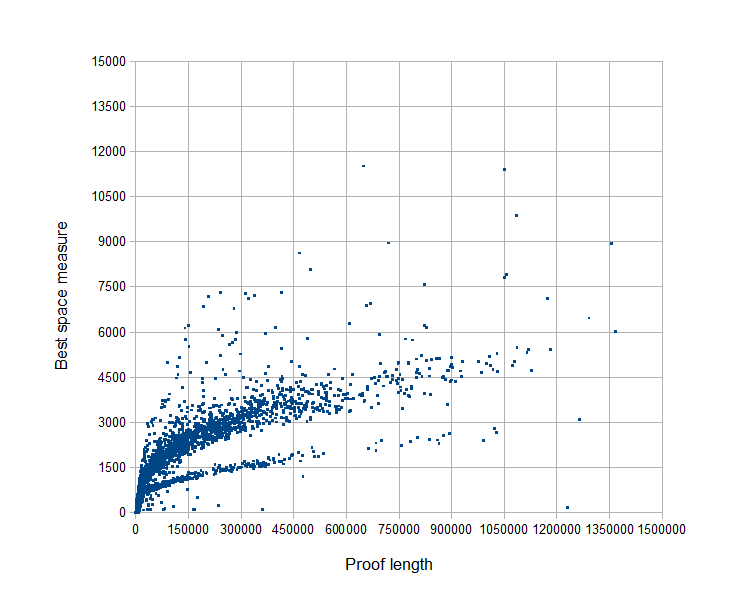
\includegraphics[scale=0.4]{Figures/length_vs_space_2.png}
	\caption{Best space measure compared to proof length}
	\label{fig:SpaceVSLength}
\end{figure}

\begin{figure}
	\centering
	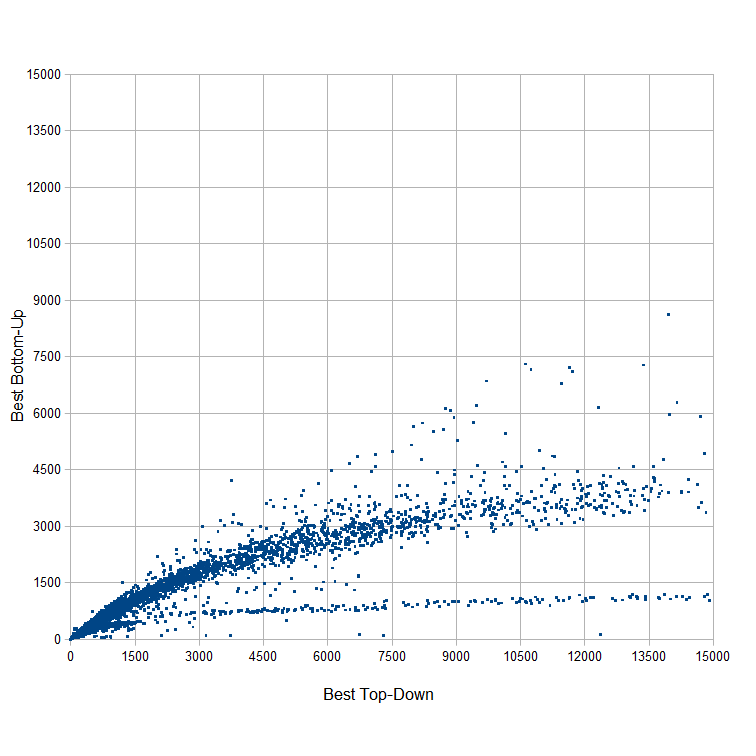
\includegraphics[scale=0.4]{Figures/TD_vs_BU-scatter_min.png}
	\caption{Spaces obtained with best \algo{Bottom-Up} and \algo{Top-Down} heuristics}
	\label{fig:BUvsTD}
\end{figure}


\begin{equation} \label{eq:space}
  \mathit{performance}(f, G, P) = \frac{1}{|P|} * \sum_{\varphi \in P}{\left( 1 -
    \frac{
      s(\varphi,f(\varphi))
    }{
        \mathit{avg}_{g\in G}{s(\varphi,g(\varphi))}
    } \right)
  }
\end{equation}

\begin{table}[tb]
	\centering
	\setlength{\tabcolsep}{8pt}
	\begin{tabular}{|l|c|c|c|}
		\hline
		\textbf{Name} & \textbf{Number of proofs} & \textbf{Maximum length} & \textbf{Average length} \\ 
		\hline \hline
		TRC1 & 2239 & 90756   & 5423   \\ \hline
		TRC2 & 215	& 1768249 & 268863 \\ \hline
    SMT1 & 4187 & 2241042 & 103162 \\ \hline
    SMT2 & 914  & 120075  & 5391  \\ 
		\hline   
	\end{tabular}
	\caption{Proof benchmark sets}
	\label{tab:benchmarks}
\end{table}

\newcommand{\cHline}{\\[-2.5ex] \hline \\[-2.5ex]}
\begin{table}[tb]
\centering
\setlength{\tabcolsep}{8pt}
\begin{tabular}{|l|c|c|c|c|c|c}
\hline
\textbf{Algorithm} & \multicolumn{4}{c|}{\textbf{Relative Performance} (\%)} & \textbf{Speed}\\ 
Heuristic:Method & \textbf{SMT1} & \textbf{SMT2} & \textbf{TRC1} & \textbf{TRC2} & (nodes/ms)\\ 
\hline\hline
Ch:BU & 19,53 & -15,79 & 20,48 & \textbf{88,57} & \textbf{88,55} \\ 
Ch:TD & \textbf{-22,07} & 8,29 & -48,33 & -67,12 & 0,30 \\ \cHline
Lc:BU & \textbf{23,42}& 36,69 & 21,47 & 88,55 & 84,43 \\ 
Lc:TD & -20,88 & 14,20 & -64,07 & \textbf{-110,00} & 1,87 \\ \cHline
Dist(1):BU & & -15,72 & 19,74 & & 21,23 \\ 
Dist(1):TD & & -67,52 & -71,21 & & 0,63 \\ 
Dist(3):BU & & -50,27 & 19,95 & & 0,54\\ 
Dist(3):TD & & \textbf{-74,90} & \textbf{-74,09} & & \textbf{0,08}\\ \cHline
Dc(LC,0.5,1,avg):BU & & 37,39 & 21,83 & & 47,70\\ 
Dc(LC,0.5,7,avg):BU & & 37,78 & 22,05 & & 14,01 \\
Dc(LC,3,1,avg):BU & & 36,86 & 22,02 & & 63,97\\
Dc(LC,3,7,avg):BU & & 34,69 & \textbf{22,55} & & 15,31 \\ 
Dc(LC,0.5,1,max):BU & & 37,31 & 21,76 & & 47,03 \\
Dc(LC,0.5,7,max):BU & & 37,89 & 21,94 & & 15,26 \\
Dc(LC,3,1,max):BU & & 37,33 & 21,79 & & 64,43 \\
Dc(LC,3,7,max):BU & & \textbf{37,96} & 22,13 & & 15,34 \\
%\bottomrule
\hline
\end{tabular}
\caption{Experimental results}
\label{tab:results}
\end{table}

\noindent
Table \ref{tab:results} shows that \algo{Bottom-Up} algorithms construct topological orders with much smaller space measures than \algo{Top-Down} algorithms. This fact is visualized in Figure \ref{fig:BUvsTD}, where each dot represents a proof $\varphi$ and the $x$ and $y$ coordinates show the space of $\varphi$ with the topological orders found by, respectively, the best \algo{Top-Down} and \algo{Bottom-Up} algorithms for $\varphi$. Some other heuristics (not described in this paper) aimed at improving \algo{Top-Down} Pebbling were tested on small benchmark sets, but none showed promising results.

Furthermore, \algo{Bottom-Up} algorithms are also much faster, as can be seen in the last column of Table \ref{tab:results}. This is so because they require fewer comparisons in their heuristic choices. For \algo{Bottom-Up} algorithms, the set $N$ of possible choices consists of the premises of a single node only, and usually $|N| \in O(1)$ (e.g. for a binary resolution proof, $N \leq 2$ always). On the other hand, the set $N$ of currently pebbleable nodes, from which \algo{Top-Down} algorithms must choose, is large (e.g. for a perfect binary tree with $2n -1$ nodes, initially $|N| = n$). For some heuristics, \algo{Top-Down} algorithms could be made more efficient by using, instead of a set, an ordered sequence of pebbleable nodes together with their memorized heuristic evaluations.

Using the \algo{Distance} Heuristic has a severe impact on the speed, which decreases rapidly as the maximum radius increases. With a radius equal to 5, only a few small proofs were processed in a reasonable amount of time.

As expected, the \algo{Decay} Heuristic does improve the results of the underlying heuristic. Note that because of the relative nature of the performance measure and the poor performance of the \algo{Top-Down} algorithms, small performance differences can still be significant. Nevertheless, the performance improvement comes at a high cost in speed.

\section{Conclusions}

Several algorithms for compressing proofs with respect to space have been conceived. The experimental evaluation clearly shows that the so-called \algo{Bottom-Up} algorithms are faster and compress more than the more natural, straightforward and simple \algo{Top-Down} algorithms. Both kinds of algorithms are parameterized by a heuristic function for selecting nodes. The best performances are achieved with the simplest heuristics (i.e. \algo{Last Child} and \algo{Number of Children}). More sophisticated heuristics provided little extra compression but cost a high price in execution time. Future work could investigate heuristics that take advantage of the particular shape of proofs generated by analysis of conflict graphs.

\vspace{-5pt}
\paragraph{Acknowledgments:} We would like to thank Armin Biere for clarifying why resolution chains are not left-associative in the TraceCheck proof format.

\vspace{-5pt}

\bibliographystyle{splncs}
\bibliography{biblio}


\end{document}

% vim: tw=100
